\documentclass{../../oss-apphys-exam}
\newcounter{last}

\begin{document}
%\genheader

\gentitle{16}{CAPACITORS}
%\genmultidirections
\raggedcolumns

\begin{multicols*}{2}
  \textbf{Questions \ref{cap1}--\ref{cap2}}

  \begin{center}
    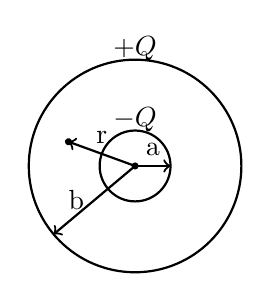
\begin{tikzpicture}[scale=.45,thick]
      \draw circle(1);
      \draw circle(3);
      \fill circle(.1);
      \draw[->](0,0)--(1,0) node[midway,above]{a};
      \draw[->,rotate=-140](0,0)--(3,0) node[midway,left]{b};
      \begin{scope}[rotate=160]
        \draw[->](0,0)--(2,0) node[midway,above]{r};
        \fill(2,0) circle(.1);
      \end{scope}
      \node at (0,3.3) (a){$+Q$};
      \node at (0,1.3) (b){$-Q$};
    \end{tikzpicture}
  \end{center}
  The spherical capacitor shown above consists of a conducting shell of
  radius $a$ inside a larger conducting shell of radius $b$. A charge $-Q$
  is placed on the inner sphere and a charge $+Q$ is placed on the outer
  shell. The capacitance of the capacitor is $C_0$.

  \begin{questions}
    \question The magnitude of the electric field $E$ at a distance $r$ between
    the spheres is
    \label{cap1}
    \begin{choices}
      \choice $\dfrac Q{4\pi\epsilon_0r^2}$
      \choice $\dfrac Q{4\pi\epsilon_0r}$
      \choice $\dfrac Q{4\pi\epsilon_0a^2}$
      \choice $\dfrac Q{4\pi\epsilon_0b^2}$
      \choice zero
    \end{choices}

    \question The bottom half of the space between the spheres is filled with
    oil of dielectric constant $\kappa=3$, creating two capacitors connected to
    each other. Which of the following is true of the two capacitors?
    \begin{center}
      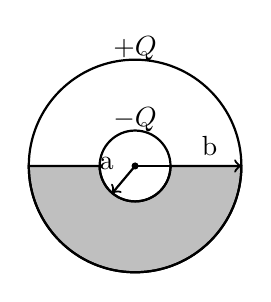
\begin{tikzpicture}[scale=.45,thick]
        \draw[fill=lightgray](-1,0)--(-3,0) arc(180:360:3)--(1,0) arc(0:-180:1);
        \draw circle(1);
        \draw circle(3);
        \fill circle(.1);
        \draw[->,rotate=230](0,0)--(1,0) node[midway,above left]{a};
        \draw[->](0,0)--(3,0) node[pos=.7,above]{b};
        \node at (0,3.3) (a){$+Q$};
        \node at (0,1.3) (b){$-Q$};
      \end{tikzpicture}
    \end{center}
    \begin{choices}
      \choice They are connected in series.
      \choice They are connected in parallel.
      \choice The total capacitance has not changed.
      \choice The total capacitance of the spheres has decreased.
      \choice The total capacitance is now zero.
    \end{choices}
    \vspace{.7in}
    \columnbreak
    
    \question With the bottom half of the space between the spheres having been
    filled with oil of dielectric constant $\kappa=3$, the new capacitance of
    the spheres is
    \label{cap2}
    \begin{choices}
      \choice zero
      \choice $C_0$
      \choice $2C_0$
      \choice $3C_0$
      \choice $4C_0$
    \end{choices}

    \uplevel{
      \textbf{Questions \ref{plate1}--\ref{plate2}}: The equation for
      determining the capacitance of a capacitor of plate area $A$ and
      separation $d$ is $C=\dfrac{\epsilon_0A}d$.
    }

    \question This equation can be derived from
    \begin{choices}
      \choice Ampere's law
      \choice Faraday's law of induction
      \choice Gauss's law for electrostatics
      \choice Gauss's law for magnetism
      \choice Ohm's law of circuits
    \end{choices}
    \label{plate1}
    \vspace{.7in}
    
    \question If a dielectric of constant $\kappa=4$ is placed between the
    plates of the capacitor and the separation between the plates is decreased
    to $d/2$, the capacitance
    \begin{choices}
      \choice increases by a factor of 4
      \choice decreases by a factor of 4
      \choice increases by a factor of 8
      \choice decreases by a factor of 8
      \choice is unchanged
    \end{choices}
    \label{plate2}
    \columnbreak
    
    \uplevel{
      \textbf{Questions \ref{cyl1}--\ref{cyl2}}: The cylindrical capacitor
      shown consists of a conducting shell of radius $a$ inside a larger
      conducting shell of radius $b$. A charge $-Q$ is placed on the inner
      sphere and a charge $+Q$ is placed on the outer shell. The length of the
      capacitor is $L$, which is very long compared to $a$ and $b$. The
      capacitance of the capacitor is $C_0$.
      \cpic{.23}{cylinder1}
    }

    \question The magnitude of the electric field $E$ at a distance $r$ between
    the cylinders is
    \begin{choices}
      \choice $\dfrac Q{4\pi\epsilon_0r^2}$
      \choice $\dfrac Q{\pi\epsilon_0rL}$
      \choice $\dfrac Q{2\pi\epsilon_0rL}$
      \choice $\dfrac Q{2\pi\epsilon_0L^2}$
      \choice zero
    \end{choices}
    \label{cyl1}
    \columnbreak
    
    \question One-third of the length of the space between the cylinders is
    filled with oil of dielectric constant $\kappa=3$, creating two capacitors
    connected to each other. Which of the following is true of the two
    capacitors?
    \cpic{.22}{cylinder2}
    \begin{choices}
      \choice They are connected in series.
      \choice They are connected in parallel.
      \choice The total capacitance has not changed.
      \choice The total capacitance of the spheres has decreased.
      \choice The total capacitance is now zero.
    \end{choices}
    \vspace{.7in}
    
    \question With one-third of the space between the cylinders having been
    filled with oil of dielectric constant $\kappa=3$, the new capacitance of
    the spheres is
    \begin{choices}
      \choice zero
      \choice $C _0$
      \choice $C_0/3$
      \choice $5C_0/3$
      \choice $4C_0$
    \end{choices}
    \label{cyl2}
  \end{questions}
  \setcounter{last}{\value{question}}
\end{multicols*}
\newpage

%\genfreetitle{16}{CAPACITORS}{3}
%\genfreedirections

\cpic{.65}{nonconcentric}
\begin{questions}
  \setcounter{question}{\value{last}}
  
  % TAKEN FROM THE 2004 AP PHYSICS C FREE-RESPONSE QUESTION E&M 1. NO CHANGES TO
  % THE QUESTION HAVE BEEN MADE
 
  \question The figure above left shows a hollow, infinite, cylindrical,
  uncharged conducting shell of inner radius $r_1$ and outer radius $r_2$. An
  infinite line charge of linear charge density $+\lambda$ is parallel to its
  axis but off center. An enlarged cross section of the cylindrical shell is
  shown above right.
  \begin{parts}
    \part On the cross section above right,
    \begin{subparts}
      \subpart sketch the electric field lines, if any, in each of regions I,
      II, and III and
      \subpart use $+$ and $-$ signs to indicate any charge induced on the
      conductor.
      \end{subparts}
    \part In the spaces below, rank the electric potentials at points $a$, $b$,
    $c$, $d$, and $e$ from highest to lowest (1 = highest potential). If two
    points are at the same potential, give them the same number.

    \vspace{.1in}
    \underline{\hspace{.2in}} $V_a$\hspace{.3in}
    \underline{\hspace{.2in}} $V_b$\hspace{.3in}
    \underline{\hspace{.2in}} $V_c$\hspace{.3in}
    \underline{\hspace{.2in}} $V_d$\hspace{.3in}
    \underline{\hspace{.2in}} $V_e$
    
    \uplevel{
      \cpic{.65}{concentric}
    }

    \part The shell is replaced by another cylindrical shell that has the same
    dimensions but is nonconducting and carries a uniform volume charge density
    $+\rho$. The infinite line charge, still of charge density $+\lambda$, is
    located at the center of the shell as shown above. Using Gauss's law,
    calculate the magnitude of the electric field as a function of the distance
    $r$ from the center of the shell for each of the following regions. Express
    your answers in terms of the given quantities and fundamental constants.
    \begin{subparts}
      \subpart $r < r_1$
      \subpart $r_1\leq r\leq r_2$
      \subpart $r > r_2$
    \end{subparts}
  \end{parts}
  \newpage
  
  % TAKEN FROM THE 2011 AP PHYSICS C FREE-RESPONSE QUESTION E&M 1.
  \question A nonconducting, thin, spherical shell has a uniform surface charge
  density $\sigma$ on its outside surface and no charge anywhere else inside.
  \begin{parts}
    \part Use Gauss's law to prove that the electric field inside the shell is
    zero everywhere. Describe the Gaussian surface that you use.
    \vspace{\stretch1}
    
    \part The charges are now redistributed so that the surface charge density
    is no longer uniform. Is the electric field still zero everywhere inside the
    shell?

    \vspace{.2in}
    \underline{\hspace{.3in}} Yes\hspace{.3in}
    \underline{\hspace{.3in}} No\hspace{.3in}
    \underline{\hspace{.3in}} It cannot be determined from the information
    given.

    \vspace{.2in}Justify your answer.
    \vspace{\stretch1}
    \newpage
    
    \uplevel{
      Now consider a small conducting sphere with charge $+Q$ whose center is at
      corner $A$ of a cubical surface, as shown below.
      \cpic{.2}{gauss-cube}
    }

    \part For which faces of the surface, if any, is the electric flux through
    that face equal to zero?

    \vspace{.2in}
    \underline{\hspace{.3in}} $ABCD$\hspace{.3in}
    \underline{\hspace{.3in}} $CDEF$\hspace{.3in}
    \underline{\hspace{.3in}} $EFGH$\hspace{.3in}
    \underline{\hspace{.3in}} $ABGH$\hspace{.3in}
    \underline{\hspace{.3in}} $BCFG$\hspace{.3in}
    \underline{\hspace{.3in}} $ADEH$

    \vspace{.2in}Explain your reasoning.
    \vspace{\stretch1}
    
    \part At which corner(s) of the surface does the electric field have the
    least magnitude
    \vspace{\stretch1}
    
    \part Determine the electric field strength at the position(s) you have
    indicated in part (d) in terms of $Q$, $L$, and fundamental constants, as
    appropriate.
    \vspace{\stretch1}
    
    \part Given that one-eighth of the sphere at point A is inside the surface,
    calculate the electric flux through face $CDEF$.
    \vspace{\stretch1}
    
  \end{parts}
  \newpage
  
  % TAKEN FROM THE 2013 AP PHYSICS C FREE-RESPONSE QUESTION E&M 1
  \uplevel{
    \cpic{.7}{cylinder}
  }
  \question A very long, solid, nonconducting cylinder of radius $R$ has a
  positive charge of uniform volume density $\rho$. A section of the cylinder
  far from its ends is shown in the diagram above. Let $r$ represent the radial
  distance from the axis of the cylinder. Express all answers in terms of $r$,
  $R$, $\rho$, and fundamental constants, as appropriate.
  \begin{parts}
    \part Using Gauss's law, derive an expression for the magnitude of the
    electric field at a radius $r<R$. Draw an appropriate Gaussian surface on
    the diagram.
    \vspace{\stretch1}
    
    \part Using Gauss's law, derive an expression for the magnitude of the
    electric field at a radius $r>R$.
    \vspace{\stretch1}
    
    \part On the axes below, sketch the graph of electric field $E$ as a
    function of radial distance $r$ for $r=0$ to $r=2R$. Explicitly label any
    intercepts, asymptotes, maxima, or minima with numerical values or algebraic
    expressions, as appropriate.

    \uplevel{
      \centering
      \begin{tikzpicture}[scale=1.2]
        \draw[very thick,->](0,0)--(5,0) node[right]{$r$};
        \draw[very thick,->](0,-2)--(0,2) node[above]{$E$};
        \draw(2,.1)--(2,-.1) node[below]{$R$};
        \draw(4,.1)--(4,-.1) node[below]{$2R$};
      \end{tikzpicture}
    }
    \newpage
    
    \part
    \begin{subparts}
      \subpart Derive an expression for the magnitude of the potential
      difference between $r=0$ and $r=R$.
      \vspace{\stretch1}
      
      \subpart Is the potential higher at $r=0$ or $r=R$?

      \vspace{.2in}
      \underline{\hspace{.3in}} $r=0$\hspace{.3in}
      \underline{\hspace{.3in}} $r=R$
    \end{subparts}
    \vspace{.4in}
    
    \part The nonconducting cylinder is replaced with a conducting cylinder of
    the same shape and same linear charge density. On the axes below, sketch
    the electric field $E$ as a function of $r$ for $r = 0$ to $r = 2R$.
    Explicitly label any intercepts, asymptotes, maxima, or minima with
    numerical values or algebraic expressions, as appropriate.

    \uplevel{
      \centering
      \begin{tikzpicture}[scale=1.2]
        \draw[very thick,->](0,0)--(5,0) node[right]{$r$};
        \draw[very thick,->](0,-2)--(0,2) node[above]{$E$};
        \draw(2,.1)--(2,-.1) node[below]{$R$};
        \draw(4,.1)--(4,-.1) node[below]{$2R$};
      \end{tikzpicture}
    }
    \vspace{\stretch1}
  \end{parts}

  %\item A parallel-plate capacitor has a capacitance $C_0$ and plate separation
%  of $d$. To dielectric slabs of constants $\kappa_1$ and $\kappa_2$, each of
%  thickness $d/2$ and having the same area as the plates, are inserted between
%  the plates as shown in the figure below. When the free charge on the plates
%  are $Q$,
%  \begin{enumerate}
%  \item find the electric field in each of the dielectric
%  \item find the potential difference between the plates
%  \item show that the new capacitance is given by:
%    $\displaystyle C=\frac{\kappa_1\kappa_2}{\kappa_1+\kappa_2}C_0$
%  \end{enumerate}
%  \pic{.2}{stacked}
%  %\vspace{\stretch{1}}

%\item Several point charges produce the equipotential lines shown.
%  \begin{enumerate}[noitemsep]
%  \item At which point on the diagram is the magnitude of the electric field
%    greatest? Explain.
%  \item Points C and D are approximately \SI{.02}{\metre} apart. Point F is
%    halfway between points C and D. What is the electric field at point F?
%  \item A \SI{5.}{\micro\coulomb} point charge is moved from point C to point
%    E, then to point D by an external force. Determine the work done by the
%    external force.
%  \end{enumerate}
%  \pic{.45}{equipotentials}
%  \vspace{\stretch{1}}

%\item A potential is given by
%  \begin{displaymath}
%    V(x,y,z)=\frac{kQ}{\sqrt{(x-a)^2+y^2+z^2}}
%  \end{displaymath}
%  \begin{enumerate}[noitemsep]
%  \item Find the components $E_x$, $E_y$ and $E_z$ of the electric field by
%    differentiating this potential function.
%  \item What simple charge distribution might be responsible for this potential?
%  \end{enumerate}
%  \vspace{\stretch{1}}
\end{questions}
\end{document}
